\mbox{}
\subsection{Activities}
A l'aide des scénarios établis lors de l'étape précédente, nous avons pu établir des diagrammes d'activités. Ces diagrammes ont pour but de modéliser les flux d'informations entre l'acteur impliqué dans le scénario et le système.
Ce diagramme nous sert pour visualiser de manière plus claire, notamment les conditions qui peuvent être rencontrées au cours d'une action.\\

Dans le cas présent, nous avons réalisé ces diagrammes afin de nous conforter dans ce que les use-case nous ont apporté, et éventuellement les compléter, car ils sont forts liés l'un à l'autre. Ceci nous a confirmé les choix effectués lors de l'établissement du schéma entité-association.

\subsubsection{L'ajout d'une personne}
\begin{figure}[H]
\centering
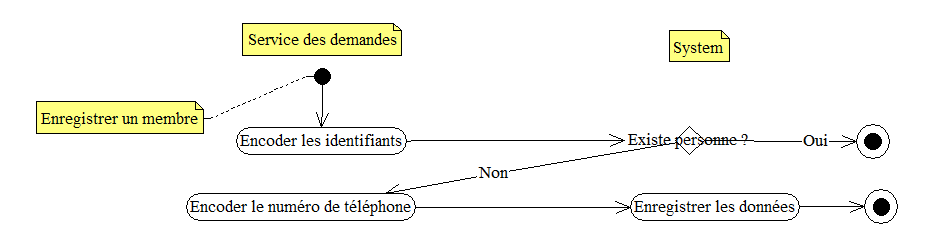
\includegraphics[width=16cm]{ajoutMembre.png}
\caption{Activity diagram de l'ajout d'une personne dans le système.}
\label{fig:ajoutMembre}
\end{figure}

Note : les identifiants de vérification  de l'unicité sont, comme mentionné dans le scénario, le nom, le prénom, et l'adresse.

\subsubsection{L'ajout d'un bien}
\begin{figure}[H]
\centering
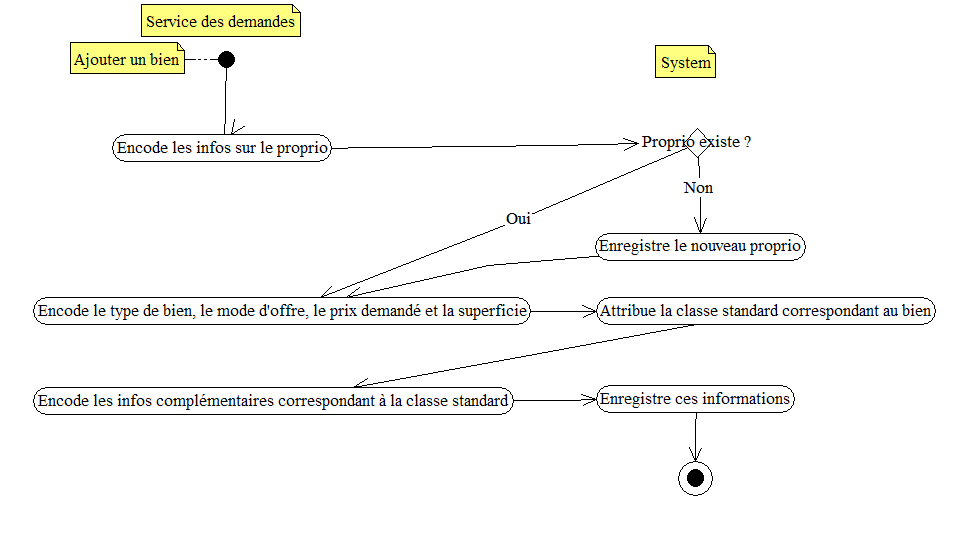
\includegraphics[width=16cm]{ajoutBien.png}
\caption{Activity diagram de l'ajout d'un bien dans le système.}
\label{fig:ajoutBien}
\end{figure}
Dans le cas présent, nous voyons clairement l'interaction de cette fonctionnalité, qui dans son mode de fonctionnement, intègre la fonctionnalité d'ajout d'un membre.

\subsubsection{La gestion de la demande d'un client}
\begin{figure}[H]
\centering
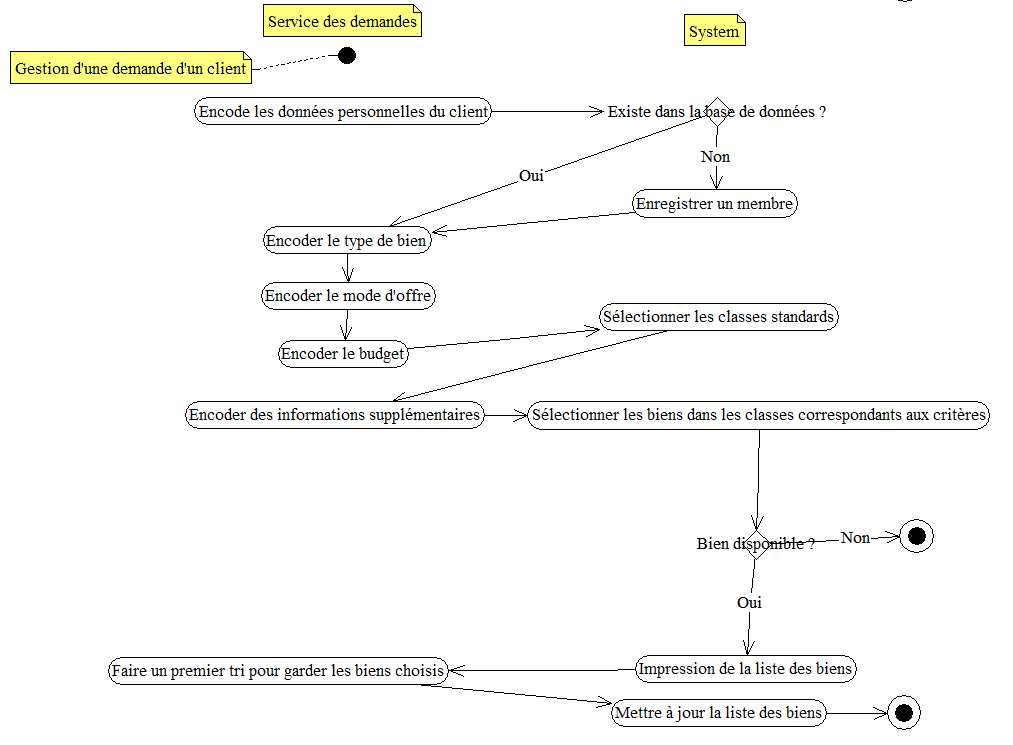
\includegraphics[width=16cm]{demandeBien.png}
\caption{Activity diagram de la demande d'un bien par un client.}
\label{fig:demandeBien}
\end{figure}
Comme dans pour le schéma d'ajout d'un bien dans le système, on voit ici clairement l'interaction entre fonctionnalités.

\subsubsection{La planification des visites}
\begin{figure}[H]
\centering
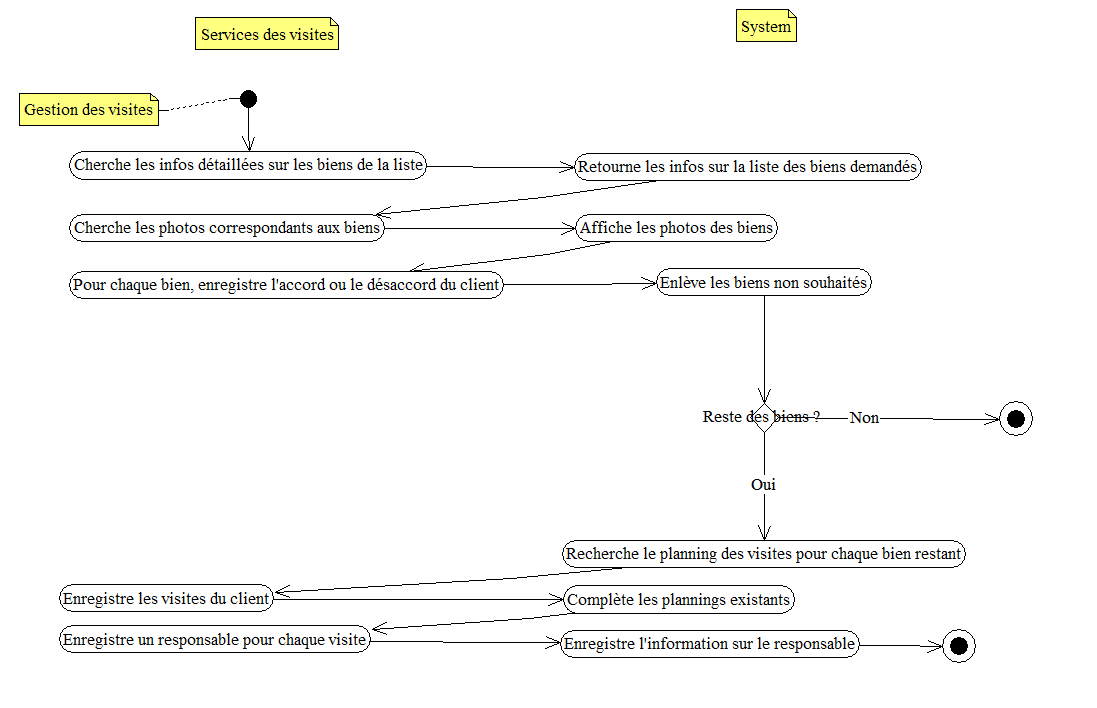
\includegraphics[width=16cm]{visites.png}
\caption{Activity diagram de l'organisation des visites.}
\label{fig:visites}
\end{figure}

\subsubsection{L'établissement d'un contrat}
\begin{figure}[H]
\centering
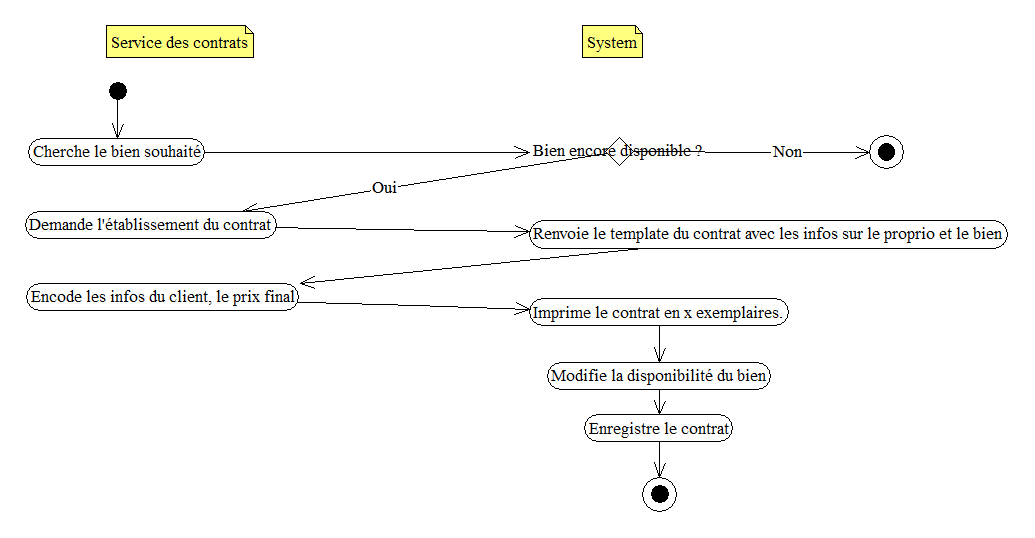
\includegraphics[width=16cm]{contrat.png}
\caption{Activity diagram de l'établissement d'un contrat.}
\label{fig:contrat}
\end{figure}

\subsubsection{La création des statistiques}
\begin{figure}[H]
\centering
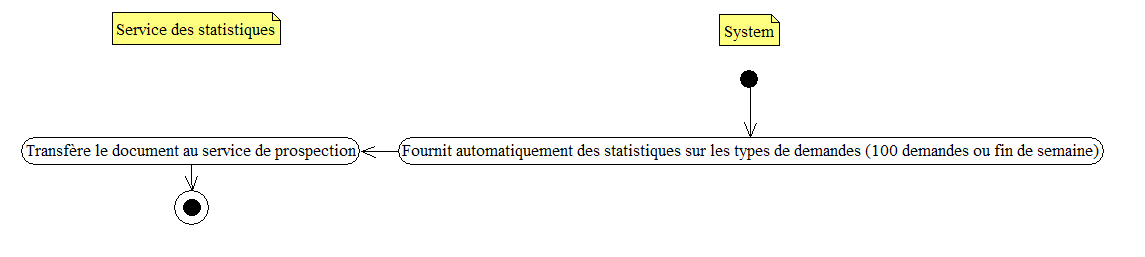
\includegraphics[width=16cm]{stats.png}
\caption{Activity diagram de la génération des statistiques.}
\label{fig:stats}
\end{figure}